% !TeX program = xelatex
% Generated from docs/workbench-walkthrough.md by scripts/build_walkthrough_latex.py.
% Compile twice with XeLaTeX for the contents and hyperlinks.
% This source is standalone; the process diagram is drawn in TikZ.
\documentclass[11pt,a4paper]{article}
\usepackage[margin=24mm,headheight=15pt,headsep=8mm,footskip=12mm]{geometry}
\usepackage{fontspec}
\usepackage{unicode-math}
\IfFontExistsTF{STIXGeneral}
  {\setmainfont{STIXGeneral}}
  {\setmainfont{Libertinus Serif}}
\IfFontExistsTF{Menlo}
  {\setmonofont[Scale=0.82]{Menlo}}
  {\setmonofont[Scale=0.86]{DejaVu Sans Mono}}
\setmathfont{STIX Two Math}
\usepackage{microtype}
\usepackage{amsmath}
\usepackage{graphicx,booktabs,longtable,array,calc}
\usepackage{fvextra}
\usepackage{newunicodechar}
\newunicodechar{⊤}{\ensuremath{\top}}
\usepackage{xcolor}
\definecolor{DSgreen}{HTML}{294F43}
\definecolor{DSmuted}{HTML}{56655F}
\definecolor{DSpale}{HTML}{F1F5F2}
\usepackage{xurl}
\usepackage[colorlinks=true,linkcolor=DSgreen,urlcolor=DSgreen,filecolor=DSgreen,
  pdftitle={DS Workbench: Complete Technical Walkthrough},
  pdfsubject={Dynamic Syntax, Classical and Constructive semantics, TTR, architecture and coverage},
  bookmarksnumbered=true]{hyperref}
\urlstyle{tt}
\usepackage{bookmark}
\usepackage{titlesec,needspace,etoolbox}
\usepackage{fancyhdr}
\usepackage{tikz}
\usetikzlibrary{arrows.meta,positioning}
\pagestyle{fancy}
\fancyhf{}
\fancyhead[L]{\small\textcolor{DSmuted}{DS Workbench}}
\fancyhead[R]{\small\textcolor{DSmuted}{Technical walkthrough}}
\fancyfoot[C]{\small\thepage}
\renewcommand{\headrulewidth}{0.3pt}
\renewcommand{\footrulewidth}{0pt}
\titleformat{\section}{\Large\bfseries\color{DSgreen}}{\thesection}{0.65em}{}
\titlespacing*{\section}{0pt}{2.0ex plus 1ex minus .2ex}{1.0ex}
\pretocmd{\section}{\Needspace{7\baselineskip}}{}{}
\setlength{\parindent}{0pt}
\setlength{\parskip}{4.5pt plus 1pt}
\setlength{\emergencystretch}{2em}
\setlength{\LTpre}{8pt}
\setlength{\LTpost}{8pt}
\BeforeBeginEnvironment{longtable}{\Needspace{13\baselineskip}}
\AtBeginEnvironment{longtable}{\small\setlength{\tabcolsep}{5pt}\renewcommand{\arraystretch}{1.16}}
\providecommand{\tightlist}{\setlength{\itemsep}{2pt}\setlength{\parskip}{0pt}}
\widowpenalty=10000
\clubpenalty=10000
\raggedbottom
\begin{document}
\begin{titlepage}
\thispagestyle{empty}
\vspace*{19mm}
{\small\color{DSmuted}\MakeUppercase{Dynamic Syntax Laboratory}\par}
\vspace{13mm}
{\fontsize{36}{41}\selectfont\bfseries\color{DSgreen}DS Workbench\par}
\vspace{4mm}
{\Large Complete technical walkthrough\par}
\vspace{9mm}
{\color{DSgreen}\rule{\linewidth}{0.7pt}}
\vspace{6mm}
{\large Syntax as the growth of transparent semantic representations\par}
\vspace{12mm}
\begin{minipage}{0.90\linewidth}
The DynamicSyntax Python package and its DyLan foundation; the engine, grammar
and application extensions built on it; Classical, Constructive and TTR
interpretations; lexical assistance, corpus integration and verification;
current limitations and a prioritized plan for broader coverage.
\end{minipage}
\vfill
{\color{DSmuted}Checked against the working source on 4 October 2026.\par}
\vspace{3mm}
\href{https://ds-workbench.vercel.app/}{ds-workbench.vercel.app}
\end{titlepage}
\pagenumbering{roman}
\tableofcontents
\clearpage
\pagenumbering{arabic}
Core walkthrough checked on 4 October 2026; research/relative-clause and
community handover updates on 7 October 2026. Public application:
\url{https://ds-workbench.vercel.app/}. This describes the implemented
system, including the TTR referent-identity correction, live Greek
lexical evidence, the controlled Jev comparison, and reusable
finite-clause construction assistance. Section 2 documents the software
foundation and additions; section 18 sets out the proposed next work.
Future work is not counted as implemented coverage. Older design
documents record earlier stages and can have outdated claims. Section 19
describes the local community handover work; it has not been published
as a separate source/package release.

\section{What the application is}\label{what-the-application-is}

DS Workbench is an interactive front end to an incremental Dynamic
Syntax parser. It displays the semantic tree after each word, and can
expose the lexical rules and individual instructions that built it. It
has three semantic families: Classical DS, Constructive DS, and DS-TTR.
Dictionary and corpus services enlarge the available vocabulary;
optional language models suggest lexical analyses, finite-clause
construction hypotheses or preferences. The DS engine constructs the
derivation.

It is presently a research and teaching workbench with an expanding
grammar fragment. It does \textbf{not yet meet the requested standard of
reliably parsing an arbitrary Greek or English paragraph}. Running a
paragraph through the interface and obtaining some complete sentences is
different from covering open text. The application retains failed
sentences and reports the distinction.

There are three independent questions when examining a result:

\begin{longtable}[]{@{}
  >{\raggedright\arraybackslash}p{(\columnwidth - 2\tabcolsep) * \real{0.3000}}
  >{\raggedright\arraybackslash}p{(\columnwidth - 2\tabcolsep) * \real{0.7000}}@{}}
\toprule\noalign{}
\begin{minipage}[b]{\linewidth}\raggedright
Question
\end{minipage} & \begin{minipage}[b]{\linewidth}\raggedright
What the application actually establishes
\end{minipage} \\
\midrule\noalign{}
\endhead
\bottomrule\noalign{}
\endlastfoot
Does each word have an entry? & Lexical coverage for this input and
selected vocabulary source. \\
Did a derivation complete? & The implemented grammar's tree requirements
were satisfied, subject to its lexical and contextual assumptions and
available semantic checks. \\
Is this the correct interpretation of grammatical language? & Completion
alone does not establish this. Lexical sense, valency, reference and the
grammar itself still require linguistic assessment. \\
\end{longtable}

The TTR bug discovered in this audit is a concrete illustration: the
tree could complete while an incorrect variable collision corrupted the
interpretation. Neither a green completion badge nor a type system
proves the Python implementation correct.

\section{Software foundation: dynamicsyntax, DyLan and our
extensions}\label{software-foundation-dynamicsyntax-dylan-and-our-extensions}

\textbf{DS Workbench extends the \texttt{dynamicsyntax} Python package},
a Python port of the Java \textbf{DyLan Dynamic Syntax parser}. The
software lineage is Java DyLan, then the Python DynamicSyntax
implementation, then the modified implementation and web application
described here. Dynamic Syntax is the linguistic framework; DyLan and
\texttt{dynamicsyntax} are software implementations of it. The system's
basis is therefore a DS parser with substantial TTR machinery, rather
than a generic TTR library to which a parser was subsequently added.

The repository's \href{../README.md}{README} credits the Java-to-Python
translation to
\href{https://github.com/incrementaliser}{@incrementaliser}. Its
\href{../pyproject.toml}{package metadata} names \textbf{Arash
Ashrafzadeh} as author of the \texttt{dynamicsyntax} distribution and
identifies the upstream repository as
\url{https://github.com/incrementaliser/DynamicSyntax}. DyLan is linked
there to the \href{https://github.com/Dynamics-of-Language}{Dynamics of
Language project}. Those credits belong to the foundation; the workbench
extensions do not imply that we originated the parser architecture or
TTR.

\textbf{Package name and implementation namespaces.} Python users import
\texttt{dynamicsyntax}; that package exposes the high-level
\texttt{parse()} and \texttt{icp()} APIs, grammar discovery and result
objects. Most engine implementation lives in the \texttt{dylan}
namespace: tree and label classes, formulas, lexical/computational
actions, parser search and the context DAG. These two namespaces are
parts of the same source distribution, not two independent parsing
servers. The alias \texttt{ttr} resolves to the bundled
\texttt{2015-english-ttr} grammar; it does not select every semantic
implementation in the application.

\textbf{What we retained and what we changed.} The inherited engine
already parsed incrementally, executed lexical actions, represented
alternatives in a DAG, manipulated TTR formulas and supported
backtracking. The repository also had GUI/web, visualization and
induction work before the current workbench. Our contribution is an
extension of that codebase, including changes to its core, rather than
just a new display around an unchanged library.

\begin{longtable}[]{@{}
  >{\raggedright\arraybackslash}p{(\columnwidth - 4\tabcolsep) * \real{0.2700}}
  >{\raggedright\arraybackslash}p{(\columnwidth - 4\tabcolsep) * \real{0.3650}}
  >{\raggedright\arraybackslash}p{(\columnwidth - 4\tabcolsep) * \real{0.3650}}@{}}
\toprule\noalign{}
\begin{minipage}[b]{\linewidth}\raggedright
Layer
\end{minipage} & \begin{minipage}[b]{\linewidth}\raggedright
Foundation retained
\end{minipage} & \begin{minipage}[b]{\linewidth}\raggedright
Workbench extensions and changes
\end{minipage} \\
\midrule\noalign{}
\endhead
\bottomrule\noalign{}
\endlastfoot
Parser and context & Incremental parser, lexical alternatives, context
DAG and repairs & Completion recovery, explicit limits, statistics,
alternative analyses and replay/state isolation fixes \\
Trees and action language & Nodes, pointer, labels, IF/THEN/ELSE,
make/go/put, MERGE and LINK machinery & Extended modal and feature
checks, unfixed-node constraints, native semantic operations and
operation-level playback \\
TTR semantics & Record types/functions, field dependencies, record
composition and English resources & Branch-local freshening,
preservation of participant constants, rejection of invalid manifests
and tests of argument identity \\
Other semantic systems & Shared DS execution framework and formula
interface & Classical lambda/choice terms and Constructive dependent
terms, nominal typing, separate semantic profiles and Constructive Coq
export \\
Grammars and vocabulary & Existing resource loader, action templates and
legacy grammars & Native English/Greek grammar resources, reviewed
clitic fragments, explicit construction families, WordNet/GDT candidates
and validated model proposals \\
Application and sources & Public Python entry points and earlier
interfaces & Current HTML/JavaScript/SVG workbench, isolated HTTP
workers, sentence/paragraph/dialogue flows, OpenRouter, Jev controls,
source evidence and deployment \\
\end{longtable}

\textbf{How the additional semantics enter the engine.}
\texttt{semantics.json} declares a native grammar's backend, axiom,
constants, predicate signatures and nominal hierarchy. Native
type/formula syntax is dispatched through the existing label and effect
factories. Trees carry the semantic profile during cloning and search.
Elimination then uses the appropriate native composition rather than TTR
record composition. The \nolinkurl{formula/mltt/} directory contains
shared native term infrastructure used by both Classical and
Constructive modes; its folder name does not mean Classical
interpretation has become Constructive. Each mode has different
permitted terms and interpretation policies. TTR remains on its own
record-semantic path. Section 4 gives concrete resulting meanings.

For example, native \texttt{a\ man\ knows\ you} executes DS actions over
the native grammar and composes a choice term or a dependent witness. It
is not obtained by running the legacy TTR grammar and renaming fields
afterward. Conversely, fixing a TTR referent collision repairs the
inherited record path; it does not make the native grammar's new
constructions available to TTR automatically.

\textbf{Evidence from the repository history.} Commit \texttt{57a6f57}
on 25 September 2026 introduces the local graphical workbench;
\texttt{4ea554a} adds the native Classical and Constructive semantic
modes; \texttt{cac8923} restores the Classical common-noun restrictor
structure. Later checkpoints include English LINK relatives
(\texttt{f53a650}), WordNet/provider integration (\texttt{064e2fc}) and
incremental lexical reconsideration (\texttt{84f28d8}). These identify
development stages, not a complete attribution of every earlier change.
The 4 October deployment also contains subsequent local changes,
including the source integration and TTR fix. \texttt{84f28d8} alone
does not reproduce that deployment: its staged hash manifest and source
snapshot are also needed. No new published PyPI release is claimed.

Installing \texttt{dynamicsyntax} from PyPI therefore does not by itself
reproduce this workbench. The deployed application uses the modified
source checkout and its grammar/data files. A reproducible workbench
release needs a pinned source revision, resource hashes and
dependency/runtime information, as proposed in section 18.

\textbf{Linguistic sources and code licensing.} The theoretical sources
are distinct from the software implementation. The Constructive
implementation is motivated by Chatzikyriakidis (2025),
\emph{Constructive Dynamic Syntax}, \textbf{Languages 10(11):269}, using
modern type theory and nominal subtyping. Greek placement and PCC work
draws on Chatzikyriakidis's 2010 thesis, especially chapters 3 and 6,
and the cited Cypriot/Pontic work. The historical panels describe
evidence and a proposal about change; they are not executable grammars
of Koine or medieval Greek. These are implemented fragments motivated by
the cited analyses, not complete implementations of every construction
discussed in those publications.

The inherited package metadata labelled the code BSD-3-Clause while
\href{../LICENSE}{LICENSE} deferred to DyLan. Inspection on 7 October
2026 found LGPLv3 in the referenced DyLan repository's
\texttt{LICENSE.txt} (commit
\nolinkurl{ac70d021e5dc0eab24f185e5a34bbca19c0fc772}). The unsupported
BSD metadata has been removed and the upstream licence text retained.
This records the conflict; terms for all later contributions still need
resolution before a public workbench release. See
\href{../THIRD_PARTY_NOTICES.md}{the provenance notices}. Code licensing
does not put WordNet, GDT, corpora or dictionary content on the same
terms; their separate conditions are discussed in section 12.

See \href{design/native-semantics.md}{the native semantic design},
\href{design/constructive-ds-design.md}{the constructive specification},
and \href{design/greek-clitics.md}{the Greek source notes}. Read their
dated sections as development history; the coverage inventory below
describes the current state.

\section{What all three implementations
share}\label{what-all-three-implementations-share}

A DS state is a tree plus a distinguished \textbf{pointer}. Addresses
identify positions: \texttt{0} is the root, \texttt{00} its argument
daughter, \texttt{01} its functor daughter. Labels include the node
address \texttt{Tn}, a type \texttt{Ty}, a formula \texttt{Fo},
grammatical features, and requirements such as \texttt{?Ty(t)} or an
unresolved formula.

The initial tree asks for a proposition. Each word selects a lexical
program. Its conditions inspect the existing state; its instructions
create nodes, move the pointer, add or remove labels, introduce
formulas, or abort that candidate. Computational rules perform
operations such as anticipation, completion, thinning satisfied
requirements, substitution, MERGE and function application.

For a simple transitive clause, subject information occupies one branch;
a verb creates or fills a function whose open object requirement is
satisfied by the next NP. Composition proceeds up the tree. The stored
alternatives allow the parser to revise an earlier lexical choice when
later input makes it fail.

The context DAG records states and transitions, including word
contributions, alternative paths and repairs. It is distinct from the
semantic tree displayed at any one step. A new speaker can continue the
same semantic tree; starting a new proposition introduces another tree
in the context.

This shared machinery does \textbf{not} imply identical trees, identical
grammars, or identical meanings across semantic systems. For example,
Classical common nouns and Constructive common-noun types have different
internal structures. The Classical and Constructive grammars are not
translations of a completed TTR parse.

\section{Classical, Constructive and TTR
meanings}\label{classical-constructive-and-ttr-meanings}

\begin{longtable}[]{@{}
  >{\raggedright\arraybackslash}p{(\columnwidth - 6\tabcolsep) * \real{0.1700}}
  >{\raggedright\arraybackslash}p{(\columnwidth - 6\tabcolsep) * \real{0.2700}}
  >{\raggedright\arraybackslash}p{(\columnwidth - 6\tabcolsep) * \real{0.2800}}
  >{\raggedright\arraybackslash}p{(\columnwidth - 6\tabcolsep) * \real{0.2800}}@{}}
\toprule\noalign{}
\begin{minipage}[b]{\linewidth}\raggedright
\end{minipage} & \begin{minipage}[b]{\linewidth}\raggedright
Classical DS
\end{minipage} & \begin{minipage}[b]{\linewidth}\raggedright
Constructive DS
\end{minipage} & \begin{minipage}[b]{\linewidth}\raggedright
DS-TTR
\end{minipage} \\
\midrule\noalign{}
\endhead
\bottomrule\noalign{}
\endlastfoot
Typical types & \texttt{e}, \texttt{t}, function types, a distinct
common-noun restrictor type & \texttt{object}, \texttt{human}, nominal
types, \texttt{Prop}, \texttt{CN}, functions, dependent Σ/Π & DS node
types together with structured record types and record functions \\
Basic representation & Lambda terms, predicates, ε/τ choice terms and
quantifier constructions & Typed terms, witnesses, projections and
dependent types & Fields for individuals, events and constraints;
dependency between fields \\
Indefinite & An ε term over a noun restrictor & A dependent
pair/witness, closed existentially in the interpretation & An individual
field constrained by a predicate field \\
Composition & Typed application and beta reduction & Typed application,
nominal coercions/projections, beta reduction and witness closure &
Record-function application, path resolution, freshening and asymmetric
record merge \\
Current assisted vocabulary & Native English and Standard Modern Greek &
Native English and Standard Modern Greek & Not implemented \\
Coq export & Not the Constructive exporter & Available for the supported
term language & Not this export path \\
\end{longtable}

\textbf{A concrete comparison.} Enter \texttt{a\ man\ knows\ you.} with
assistance off. The native implementations produce:

\begin{Verbatim}[fontsize=\small,breaklines=true,breakanywhere=true,commandchars=\\\{\},frame=single,rulecolor=\color{DSmuted},framesep=5pt]
Classical:
  know(ε x0:e. man(x0), you)

Constructive, raw:
  Σ p00:(Σ x:man. \ensuremath{\top}). know(π₁(p00), you)

Constructive, simplified:
  Σ x:man. know(x, you)
\end{Verbatim}

The Constructive indefinite provides a witness \texttt{p00}. Its first
projection supplies the individual to the verb. The final interpretation
closes the witness. An interpretation type is not itself a constructed
proof that the assertion is true.

After the freshening correction, the corresponding TTR record contains
these fields, shown in a readable order without changing their names:

\begin{Verbatim}[fontsize=\small,breaklines=true,breakanywhere=true,commandchars=\\\{\},frame=single,rulecolor=\color{DSmuted},framesep=5pt]
[ x0 : e
| p0 == man(x0) : t
| x1 == you : e
| e0 == know : es
| p2 == pres(e0) : t
| p5 == subj(e0, x0) : t
| p4 == obj(e0, x1) : t
| head == e0 : es ]
\end{Verbatim}

\texttt{x0} supplies the subject and \texttt{x1} the object. \texttt{e0}
supplies the knowing event; the remaining fields constrain its tense and
participants. Display order and fresh field names are implementation
details; the dependencies are essential. Different field names do not
assert that the referents must denote distinct people: two fields may
deliberately have the same manifest individual.

TTR is itself a dependent type-theoretic framework. Calling one menu
option ``Constructive'' does not mean TTR is intrinsically
nonconstructive. The labels identify different implemented semantic
calculi.

\textbf{Important native details.} Classical determiner phrases use an
explicit common-noun restrictor structure, not just a flat predicate
pasted onto an entity. Constructive common nouns inhabit the grammar's
\texttt{CN} universe, with nominal inclusions used during application.
Satisfying a pending tree type requirement is kept distinct from
checking whether a function can consume a particular argument. Function
domains require the appropriate variance rules.

Definites need contextual assumptions. Constructive output such as
\texttt{definite\_s1\_010} names an assumed referent at a sentence/node
position; it is not evidence that the app identified the uniquely
intended door in the world. The interface displays the assumptions.

The existential-scope control supports a particular universal/indefinite
configuration, for example \texttt{Π\ doctor.\ Σ\ patient.\ ...} versus
\texttt{Σ\ patient.\ Π\ doctor.\ ...}. It changes the supported closure
policy; it does not enumerate every possible natural-language scope
reading.

Finite complements have local witness closure. Constructive embedded
contents use a \texttt{Content} representation exported as a Coq type.
The attitude predicates remain opaque: there is no general logic of
belief, factivity or possible worlds.

\section{The TTR defect found and
corrected}\label{the-ttr-defect-found-and-corrected}

Previously \texttt{ttrput} passed the live dialogue \texttt{Context} to
a freshening method that expected a \texttt{Tree} or parser tuple. The
record implementation silently returned an unchanged clone for an
unsupported argument. Both noun phrases therefore retained the field
name \texttt{x}.

Later composition correctly followed the implemented asymmetric-merge
operation, but the inputs incorrectly reused a label. One field
overwrote the other. In \texttt{a\ man\ knows\ you}, \texttt{you}
disappeared and both participant constraints referred to \texttt{x}.
That is an implementation error, not a consequence required by TTR.

The correction allocates fresh names from \textbf{the actual branch
receiving the formula}. Each cloned branch carries its own variable
pools. Using the source tree held by the context would also be wrong
during speculative search, because it would mutate the allocator shared
by sibling alternatives. Unsupported freshening arguments now raise a
descriptive error instead of doing nothing.

Regression tests inspect participant dependencies and retained
individual constants in all three full bundled English TTR grammars.
They cover two indefinites, name reversal, repeated names,
speaker-dependent \texttt{you}, repair, repeated requests and agreement
between the final playback channels. Browser checks inspect the
displayed record and JSON export. These tests do not certify the entire
TTR port or all legacy grammar resources.

Earlier smoke tests checked successful parsing and predicate presence;
two other tests explicitly froze the corrupted record or its shared
participant variable. Those expectations have been corrected. The new
tests assert semantic relationships, including who fills each argument
role.

The audit also found that re-reading a record with a capitalized
participant constant such as \texttt{A} could discard its manifest
value. Such constants now parse, while reserved metavariables retain
their meaning. An unparseable manifest is rejected rather than converted
into an unconstrained field. Unsupported \texttt{ttrput} formulas are
rejected rather than installed as opaque semantics.

\section{Walking through the
interface}\label{walking-through-the-interface}

Start with \textbf{Sentence}, choose the semantic system and then its
grammar. Use a small known example first. With a native grammar, select
the grammar vocabulary alone to isolate the reviewed entries, or
dictionary/corpus candidates to permit deterministic lexical expansion.
Neither needs an LLM.

Press \textbf{Build derivation}. The results distinguish parser
completion, lexical coverage and independent grammaticality evidence. A
missing word means no usable lexical entry was available. A known word
can still fail because its action conditions do not fit the current
tree. Consuming every token can leave an incomplete tree with unresolved
requirements.

The playback controls expose three views:

\begin{longtable}[]{@{}
  >{\raggedright\arraybackslash}p{(\columnwidth - 2\tabcolsep) * \real{0.3000}}
  >{\raggedright\arraybackslash}p{(\columnwidth - 2\tabcolsep) * \real{0.7000}}@{}}
\toprule\noalign{}
\begin{minipage}[b]{\linewidth}\raggedright
View
\end{minipage} & \begin{minipage}[b]{\linewidth}\raggedright
What it shows
\end{minipage} \\
\midrule\noalign{}
\endhead
\bottomrule\noalign{}
\endlastfoot
Words & Recorded parser states at word boundaries. \\
Rules & The selected lexical/computational actions replayed through the
engine. \\
Operations & Individual effects such as \texttt{make}, \texttt{go},
\texttt{put}, \texttt{delete}, MERGE or reduction where replay is
available. \\
\end{longtable}

These are not three different parsing algorithms. The engine supplies
the word states; replay provides a finer explanation of the chosen path.
Some legacy transitions cannot be replayed instruction by instruction
and are explicitly grouped. The word-boundary state remains
authoritative. The trace is not a complete debugger recording every
explored and abandoned search branch.

Rules is now the default playback view. Lexical and computational
programs carry separate badges; the active rule, pointer movement and
changed decorations appear above the tree. Assisted sentences and
paragraphs stream rule transitions too. Each assisted retry starts a
separate, numbered replay; paragraph events identify the sentence they
belong to. These modes retain rule-level snapshots without the larger
primitive-operation trace. The classification comes from the executed
action class, not a model's account of what the parser did. This display
adds no model requests.

Click a node to inspect its full labels, formula and open requirements.
Node types wrap to remain visible. Long formulas can be expanded in the
tree; this only changes presentation and makes no model or parser
request. Pan, zoom and Fit help with larger trees. Playback retains the
pointer and changed-node cues.

The meaning panel follows the selected state. A partial root formula is
not a complete interpretation. The Constructive panel can also display a
simplified term. If more complete analyses were requested, the reading
selector changes the tree, meaning and corresponding export together.

\textbf{Export JSON} preserves result data, lexical provenance,
available trace and context. \textbf{Export Coq} emits the supported
Constructive meaning and its declarations. Local tests can compile these
files when \texttt{coqc} is installed; the public server does not run
Coq. Compilation establishes type correctness of the exported
representation, not a proof that the input sentence is true.

\section{What the LLM does, and what works without
it}\label{what-the-llm-does-and-what-works-without-it}

Without an LLM, the application already has the parser, grammar
programs, semantic compilers, reviewed lexical entries, bundled
morphology, WordNet, Greek corpus hypotheses, source search, playback
and exports. A dictionary candidate is still a hypothesis about which
sense/frame fits the sentence. For example, WordNet can supply many
senses of \texttt{enter}; it does not thereby choose the intended one.

With OpenRouter assistance, the sequence is:

\begin{figure}[htbp]
\centering
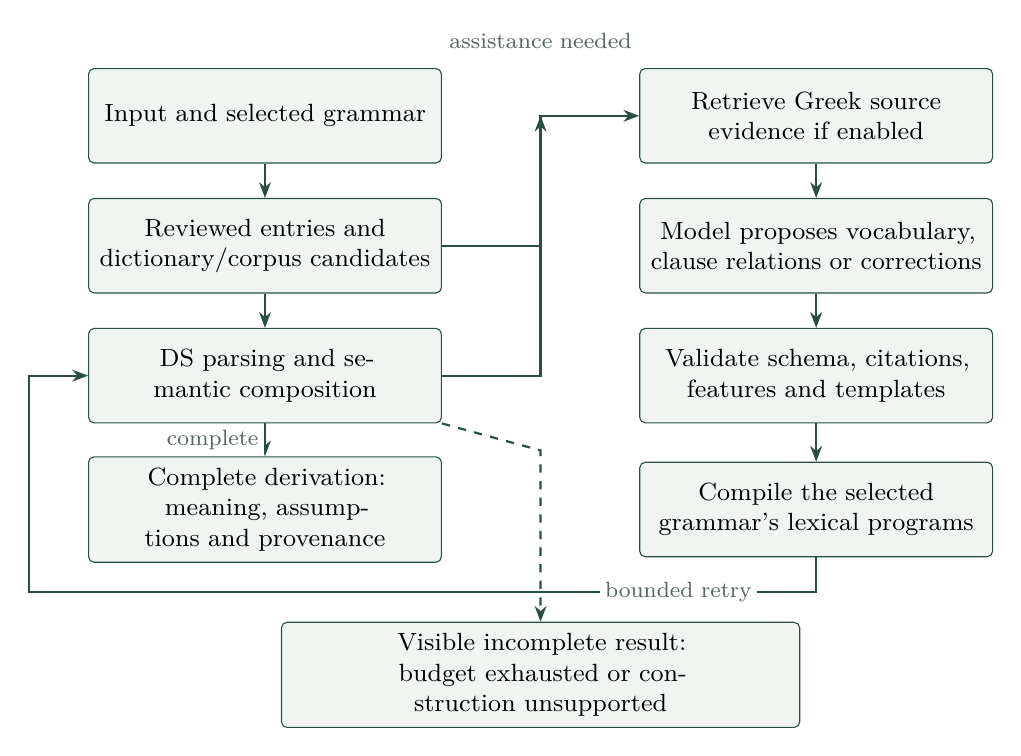
\begin{tikzpicture}[
  box/.style={draw=DSgreen,rounded corners=2pt,fill=DSpale,
    text width=42mm,minimum height=12mm,align=center,inner sep=4pt,font=\small},
  edge/.style={-{Stealth[length=2mm]},draw=DSgreen,thick},
  note/.style={font=\footnotesize,fill=white,inner sep=2pt,text=DSmuted}]
\node[box] (input) at (0,0) {Input and selected grammar};
\node[box] (entries) at (0,-1.65) {Reviewed entries and dictionary/corpus candidates};
\node[box] (ds) at (0,-3.30) {DS parsing and semantic composition};
\node[box] (success) at (0,-5.00) {Complete derivation:\\meaning, assumptions and provenance};
\node[box] (sources) at (7,0) {Retrieve Greek source evidence if enabled};
\node[box] (model) at (7,-1.65) {Model proposes vocabulary, clause relations or corrections};
\node[box] (validate) at (7,-3.30) {Validate schema, citations, features and templates};
\node[box] (compile) at (7,-5.00) {Compile the selected grammar's lexical programs};
\node[box,text width=63mm] (failure) at (3.5,-7.10) {Visible incomplete result:\\budget exhausted or construction unsupported};
\draw[edge] (input) -- (entries);
\draw[edge] (entries) -- (ds);
\draw[edge] (ds) -- node[note,left] {complete} (success);
\draw[edge] (entries.east) -- (3.5,-1.65) -- (3.5,0) -- (sources.west);
\draw[edge] (ds.east) -- (3.5,-3.30) -- (3.5,0);
\node[note,text width=24mm,align=center] at (3.5,0.95) {assistance needed};
\draw[edge] (sources) -- (model);
\draw[edge] (model) -- (validate);
\draw[edge] (validate) -- (compile);
\draw[edge] (compile.south) -- (7,-6.05) -- (-3,-6.05) -- (-3,-3.30) -- (ds.west);
\node[note] at (5.25,-6.05) {bounded retry};
\draw[edge,dashed] (ds.south east) -- (3.5,-4.25) -- (failure.north);
\end{tikzpicture}
\caption{Missing vocabulary can trigger assistance before the first DS attempt;
an incomplete derivation can trigger a correction. Optional Greek retrieval
supplies evidence for the proposal. Compilation and DS execution still determine
whether a derivation completes. Calls and retries are bounded.}
\end{figure}

The selected chat model can propose a lemma, word class, sense, nominal
domain, argument frame, morphological features or a finite-clause
relation. It receives context and, on a retry, information about the
actual failed derivation. The compiler instantiates an allowed action
template for the selected semantic backend. The model does not submit
arbitrary Python, arbitrary DS programs, or an unchecked final tree for
display as a verified parse.

The helper can request missing vocabulary before the first DS attempt as
well as corrections after a failed attempt. Optional Greek source
retrieval precedes the corresponding model proposal; it does not wait
for a successful derivation.

Validation checks the permitted fields, word forms, domains, arity and
template constraints. Predicate identifiers are controlled/generated.
Protected function words cannot simply be replaced by a content-word
guess. Existing alternatives remain available. A valid batch is
installed and DS runs again.

The construction interface separates surface words from reusable DS
operations. Twelve declared relations cover cause, temporal relations,
conditions, exceptions, concession and contrast. Common connectives
already work without AI. The model can prefer a contextual reading of
ambiguous \texttt{since}, \texttt{while}, \texttt{as}, \texttt{once},
\texttt{ενώ} or \texttt{αφού}, or propose a previously absent
lexicalization such as conditional \texttt{provided} or causal
\texttt{καθότι}. Missing-word requests accept both content-word and
construction hypotheses, so an unfamiliar conjunction does not have to
be forced into a noun/verb schema. A failed derivation can trigger a
targeted construction request. The compiler validates requested
surfaces, relation IDs, reviewed readings and signatures, then
instantiates loaded templates. It does not execute generated code or add
arbitrary types.

All original programs remain available; model preferences affect their
order. The panel \textbf{How the clauses were connected} shows
proposals, explanations, compiled programs and the relation on the
actual DS path separately. A model preference may not be used.
Known-word preferences reset between paragraph sentences; new
lexicalizations remain request-local hypotheses and are marked as reused
when appropriate. Repeated ambiguous surfaces within one sentence retain
normal DS alternatives because occurrence-specific model ranking is not
implemented. Jev remains the separate incremental lexical-sense
selector; this construction interface uses the user's selected chat
model and full context.

This explains both the usefulness and the limits of assistance. It can
supply a missing lexical item, improve a valency hypothesis, or
instantiate an existing construction with another connective. It cannot
conjure an unimplemented relative construction, auxiliary system,
reflexive-binding rule or PP attachment procedure. Those require grammar
implementation. Even a compiled lexical proposal can select the wrong
sense or frame while producing a type-compatible derivation.

Open-text mode makes at most three provider calls per request, shared
across a paragraph, with bounded DS retries. The helper has a 48-second
budget and a vocabulary call can use up to 22 seconds and a
construction-only call up to 16 seconds within the remaining allowance.
Combined requests count once. Rate limits such as HTTP 429 can stop
further model calls; remaining usable entries can still be tried by DS.
The UI reports actual model use and unresolved gaps.

This assistance can inspect the available full text. It is therefore not
an experiment in strictly prefix-only online human language processing,
even though DS builds its trees incrementally.

\textbf{Connecting.} Open Vocabulary \& AI, enter an OpenRouter key,
connect, choose a model, and choose the corresponding vocabulary mode.
Connection checks the key and obtains compatible model information; it
does not itself parse with a model. The listed model inventory and
prices come from the provider and can change. The selected model is used
for the supported vocabulary requests.

The key is held in the tab's JavaScript memory, not local storage or
exported results. It goes to the DS backend for that request and onward
to OpenRouter; the application does not persist it. Refresh or
disconnect clears the tab's copy. Inference is billed to the user's
provider account. Free application hosting does not make model calls
free.

Assistance is implemented for native English and Standard Modern Greek.
It is not implemented for TTR or generally for the other Greek
varieties. Dialogue does not run the paragraph/sentence assisted retry
pipeline.

\section{Jev is a separate optional
path}\label{jev-is-a-separate-optional-path}

Jev is used as a typed preference service over lexical alternatives and
parser state, not as the selected general chat model. The current
provider pin is \nolinkurl{typesafe/jev-1.13-20260917} on OpenRouter.
Choosing another analysis model does not silently change that pin.

Its incremental lexical path uses the observed prefix, candidate
information and current tree to prefer a sense. DS still checks frames
and every proposed revision. Alternatives remain available for
backtracking; a failed revision restores the previous path. Calls and
reconsiderations are bounded, including an eight-fresh-request parse
budget in the decision client.

\textbf{A visible comparison.} Open \textbf{See Jev in action}, connect
OpenRouter, and try \texttt{John\ lends\ a\ book\ to\ Mary.} in English
Classical or Constructive DS. The application executes two DS parses:
one with normal lexical ordering and one with Jev preferences and
reconsideration. The two result panels show the selected dictionary
glosses, composed meanings, completion status and search statistics.
Expand a decision to see the words observed, the entire probability
distribution including \texttt{uncertain}, confidence, latency,
available reported cost and any provider error. \textbf{Watch this
revision} jumps to the corresponding backtrack in the actual DS action
playback. JSON export retains the comparison.

The 4 October live check produced the following result in both native
backends:

\begin{longtable}[]{@{}
  >{\raggedright\arraybackslash}p{(\columnwidth - 2\tabcolsep) * \real{0.3000}}
  >{\raggedright\arraybackslash}p{(\columnwidth - 2\tabcolsep) * \real{0.7000}}@{}}
\toprule\noalign{}
\begin{minipage}[b]{\linewidth}\raggedright
Point in the example
\end{minipage} & \begin{minipage}[b]{\linewidth}\raggedright
Observed behaviour
\end{minipage} \\
\midrule\noalign{}
\endhead
\bottomrule\noalign{}
\endlastfoot
DS without Jev & Completed with the dictionary sense of \texttt{lend}
meaning ``bestow a quality on'' \\
Jev at \texttt{John\ lends} & Chose \texttt{uncertain}; neither object
nor recipient had been supplied \\
Jev after \texttt{John\ lends\ a\ book} & Preferred ``give
temporarily''; bounded DS replay found no compatible continuation yet
and retained the current tree \\
Jev after \texttt{John\ lends\ a\ book\ to\ Mary} & DS replay accepted
the preferred sense; the final formula used the temporary-transfer
predicate with book and Mary arguments \\
\end{longtable}

Both runs completed, so completion alone would have missed the lexical
problem. The ordinary reading of the sentence supports the
temporary-transfer choice; this is one inspected demonstration, not a
measured general improvement. There were three fresh Jev calls per
backend. Outcomes can differ on later requests. The crane example
permits reconsideration after later context, while the bank example
deliberately leaves the sense underdetermined. The interface also
reports unchanged choices, unavailable answers and incomplete
comparisons. Model probabilities are preferences, not calibrated
linguistic accuracy.

A later check on the deployed site again changed the final sense in both
backends. Classical Jev remained uncertain after \texttt{a\ book} on
that request; both accepted the revision after \texttt{to\ Mary}. The
\href{../data/lexical-revision/jev-comparison-live-2026-10-04.json}{recorded
public result} retains the actual distributions and replay outcomes. The
interface displays each request's result rather than fixed demonstration
answers.

\textbf{How the comparison is controlled.} \nolinkurl{jev_comparison.py}
prepares candidates once, including any permitted lexical-model
fallback, and copies their source programs, metadata and semantic
profile into two fresh parsers. It verifies a content hash of each
installed inventory and resets the pooled metavariable bindings between
runs. Both receive the same grammar, initial context, scope and entry
limit. The baseline does not call Jev. This matters because ordinary
dictionary mode consults the bundled extension before WordNet, whereas
Jev vocabulary mode consults WordNet first: switching those modes would
change more than the model preference. The comparison therefore uses the
Jev-mode inventory in both runs. It is not an off/on comparison of two
different vocabulary sources.

The request option is \texttt{compare\_jev:\ true} with
\texttt{lexical\_mode:\ "jev"}, normal search ordering and one requested
analysis. It currently supports native English sentences only, not
Greek, TTR, paragraphs or dialogue. The baseline has a four-second
search allowance and runs without the animation replay overhead; the
comparison has a 50-second internal budget after initial preparation
starts. Its timings are consequently not a speed benchmark. If either
run fails or times out, the comparison is inconclusive. The primary
displayed tree is the Jev run; the baseline includes its selected
entries, formula and derivation action names. The request cannot supply
arbitrary lexical programs through this internal inventory-copying
interface.

Lexical preferences and \textbf{search ordering} are separate controls.
Search-order use has calibration gates tied to the grammar, code,
provider/model and state representation. A configured key is not
evidence that ordering is enabled or beneficial. Existing experiments
did not demonstrate a backtracking benefit sufficient to enable those
gates. The normal DS ordering remains meaningful and available without
Jev.

The distinctions are thus: DS determines whether a path completes; the
chat model proposes vocabulary and finite-clause relations; Jev can
influence lexical-sense preferences among candidates. Neither service is
an independent judge of natural-language grammaticality.

\section{PP arguments, LINK modifiers and
similes}\label{pp-arguments-link-modifiers-and-similes}

Your distinction between arguments and LINK modifiers matters. The
implementation has separate cases rather than one generic
``preposition'' analysis:

\begin{longtable}[]{@{}
  >{\raggedright\arraybackslash}p{(\columnwidth - 4\tabcolsep) * \real{0.2700}}
  >{\raggedright\arraybackslash}p{(\columnwidth - 4\tabcolsep) * \real{0.3650}}
  >{\raggedright\arraybackslash}p{(\columnwidth - 4\tabcolsep) * \real{0.3650}}@{}}
\toprule\noalign{}
\begin{minipage}[b]{\linewidth}\raggedright
Use
\end{minipage} & \begin{minipage}[b]{\linewidth}\raggedright
Structural treatment
\end{minipage} & \begin{minipage}[b]{\linewidth}\raggedright
Example
\end{minipage} \\
\midrule\noalign{}
\endhead
\bottomrule\noalign{}
\endlastfoot
Selected PP argument & A lexical frame opens a required slot; the
selected preposition fills that slot & \texttt{relies\ on\ Mary}; a
reviewed goal frame for Greek \texttt{μπήκε\ στην\ πίστα} \\
Optional VP/clause modifier & A LINK structure grows and combines its
contribution with the host & Postverbal locative/manner/path modifiers
in the supported fragment \\
Copular PP predicate & The PP supplies the predicate of the subject &
\texttt{a\ man\ is\ in\ the\ room} \\
Nominal comparison & A LINK contribution uses a noun description as a
comparison standard & \texttt{like\ a\ wild\ peacock} /
\texttt{σαν\ άγριο\ παγώνι} \\
\end{longtable}

A selected argument contributes to the verb's valency. Removing it may
leave the selected frame incomplete. A modifier adds information to an
otherwise available predication. The distinction is encoded by lexical
frames and action templates; it is not reliably inferred just from the
surface preposition.

The English motion example can compose a path modifier and then a
comparison:

\begin{Verbatim}[fontsize=\small,breaklines=true,breakanywhere=true,commandchars=\\\{\},frame=single,rulecolor=\color{DSmuted},framesep=5pt]
George walks onto the stage like a wild peacock.

manner_like(Σ x:peacock. wild(x),
            onto_goal(definite_01L10, walk(george)))
\end{Verbatim}

The Greek example uses its selected goal frame:

\begin{Verbatim}[fontsize=\small,breaklines=true,breakanywhere=true,commandchars=\\\{\},frame=single,rulecolor=\color{DSmuted},framesep=5pt]
Ο Γιώργος μπήκε στην πίστα σαν άγριο παγώνι.

manner_like(Σ x:peacock. wild(x),
            enter_goal(giorgos, definite_010))
\end{Verbatim}

Here the Σ expression supplied to the comparison operator is a
\textbf{description type}, not a claim that a particular wild peacock
exists in the discourse. The construction also does not assert that
George is a peacock. Greek singular case/gender constraints are checked
by the supported nominal templates.

The semantics of \texttt{manner\_like}, path and location operators is
deliberately limited. There is no complete event/spatial theory behind
them. General NP attachment, all instrumental/comitative distinctions,
arbitrary PP chains, referential or plural comparison standards and
clausal comparisons remain outside the implemented inventory. English
and Greek have explicit related implementations; they are not obtained
by merely translating words.

\section{Current construction
coverage}\label{current-construction-coverage}

\textbf{Native English.} The maintained fragment includes names and
pronouns; indefinites, definites and universals; distributive
\texttt{all} with supported plural nouns; nominal, adjectival and
locative copulas; degree expressions; intersective attributive
adjectives; active intransitive, transitive and selected ditransitive/PP
frames; do-support negation; positive modals with supported bare verbs;
clause and VP coordination; LINK adverb/PP modifiers; finite complements
and causal clauses; and restrictive relatives with supported subject or
direct object gaps. Relatives use LINK and an unfixed head copy, with
MERGE and nominal refinement in the Constructive implementation.

\textbf{Reusable finite clauses.} A shared, parameterized construction
now covers English \texttt{when}, \texttt{whenever}, \texttt{while},
\texttt{before}, \texttt{after}, \texttt{since}, \texttt{until},
\texttt{if}, \texttt{unless}, \texttt{although}, \texttt{though},
\texttt{whereas}, \texttt{once} and \texttt{as}, and Standard Greek
\texttt{όταν}, \texttt{όποτε}, \texttt{ενώ}, \texttt{αφού},
\texttt{αν/εάν}, \texttt{μολονότι}, \texttt{παρότι},
\texttt{ωσότου/ώσπου}. Ambiguous connectives retain distinct readings.
These entries require finite clauses; they do not supply
interrogative/relative when, nominal after, gerund complements, or
multiword markers. A postposed clause uses LINK; a preposed clause
requires a comma and another clause. For example:

\begin{Verbatim}[fontsize=\small,breaklines=true,breakanywhere=true,commandchars=\\\{\},frame=single,rulecolor=\color{DSmuted},framesep=5pt]
When George opened the door, Mary entered the room.
John walks although Mary walks later.
If Bill shouts, John walks because Mary walks.
\end{Verbatim}

Both native backends parse this three-sentence paragraph without an LLM.
The last sentence composes
\texttt{condition(because(walk(john),\ walk(mary)),\ shout(bill))}. A
separate three-sentence Greek check with όταν, παρότι and αν also
completes in both backends. These are hand-written construction checks,
not a new held-out accuracy measurement.

All relations order their arguments \texttt{(main,\ subordinate)} and
preserve local content closure. They are explicit, opaque predicates.
Temporal precedence, overlap, conditions and concessions are distinct
from cause, but full event semantics, temporal anchoring,
counterfactuals and discourse inference remain unimplemented. In
particular, \texttt{condition} is not automatically material
implication. Constructive Coq exports declare
\texttt{Type\ -\textgreater{}\ Type\ -\textgreater{}\ Prop}; Classical
uses its own proposition and choice-term semantics. No TTR translation
is used.

\textbf{Causal instance.} English \texttt{because} and Standard Greek
\texttt{επειδή\ /\ διότι} now connect finite clauses in the two native
backends. Both \texttt{John\ walks\ because\ Mary\ walks\ later.} and
\texttt{Because\ Mary\ walks\ later,\ John\ walks\ today.} run without a
model. The preposed construction requires a comma and a following main
clause. Postposed reasons grow a LINK. Preposed reasons occupy a content
argument of a curried causal operator; that slot belongs to the
connective, not to the verb's lexical valency. This is the implemented
analysis, not a claim that every DS account must use that
representation.

The reported sentence
\texttt{George\ opened\ the\ door\ because\ he\ came\ later} completes
with WordNet vocabulary and no model request, in both native backends.
It also completed in live Jev mode, which retained the same lexical
choices in the check. The Constructive result has the form
\texttt{because(open(george,\ definite\_door),\ later(come(george)))},
with the actual selected WordNet predicate identifiers retained in the
export. Classical instead uses its definite choice term for the door.
The antecedent choice for \texttt{he} is the existing
most-recent-compatible-name heuristic; that assumption is now displayed.

\texttt{because(main,\ reason)} is an opaque relation between two
locally closed clause contents. It is not reduced to conjunction, and
does not supply causal inference or truth axioms. Constructive witnesses
close separately inside each content; its Coq declaration is
\texttt{because\ :\ Type\ -\textgreater{}\ Type\ -\textgreater{}\ Prop}.
Classical retains its own \texttt{t} contents and choice terms. Missing
reasons, missing main clauses and unlicensed \texttt{because\ of}
phrases remain incomplete. Supported nested reasons and
finite-complement attachments can produce separate readings.
Coordination and negation do not have a complete causal-scope calculus.

Temporal words include \texttt{later}, \texttt{earlier}, \texttt{late},
\texttt{early}, \texttt{today}, \texttt{yesterday}, \texttt{tomorrow},
\texttt{soon} and their maintained Greek counterparts. Each contributes
a distinct operator. Comparative/reference times and calendar anchoring
remain contextual; a past surface form still does not provide a full
tense/aspect interpretation. The causal addition is tested at the level
of meaning as well as completion: following adverbs/PPs cannot erase the
reason, and a modifier in a preposed reason must propagate before the
comma opens the main clause.

The dialogue work adds do/does/did polar questions, local subject-bound
reflexives and Yes/No answers to an immediately preceding complete
question. This does not provide a complete English auxiliary, tense or
question grammar.

\textbf{Standard Modern Greek.} The maintained native grammars combine a
clitic fragment with copulas, degree predication, singular case-bearing
common-noun DPs/adjectives, corpus-supported ordinary finite verbs,
destination PPs and nominal comparisons. The clitic work includes
accusative/genitive forms, person-sensitive restrictions,
monotransitives/ditransitives, imperative clusters and strong PCC
constraints. Negation, \texttt{να}, future particles and gerunds have
explicit entries. Case-marked names permit supported SVO/VSO/OVS
patterns, basic clitic coreference/doubling and restricted initial
topics.

For \texttt{της\ τον\ έδωσε}, the corpus expansion can propose a
ditransitive entry; the grammar links the accusative to the theme and
genitive to the recipient, giving \texttt{give(pro,\ him,\ her)} under
its context assumptions. A corpus observation of a transitive use of the
same lemma is not enough by itself to infer this three-place frame. The
builder records separate form and frame evidence where it combines
observations.

\textbf{Greek varieties.} Cypriot, Pontic and Grico are smaller,
separately reviewed fragments available in the native semantic families.
They model selected placement environments and restrictions, not general
dialect understanding. Cypriot supports a bare-clause/trigger contrast;
Pontic uses the reviewed postverbal conditions; maintained Grico work
includes selected cluster order and PCC behaviour. The interface's
source and environment qualifications are part of the analysis. A
sentence outside the reviewed inventory cannot be treated as evidence
against the dialect's grammar.

\textbf{Legacy TTR English.} The bundled resources retain their own
lexicon and construction inventory. Native English additions are not
automatically added to these files. Some legacy entries fail non-strict
loader validation and are skipped with warnings. A row visible in a
lexicon file therefore does not prove the word/action is usable. The
small \nolinkurl{2026-english-ttr-test} resource is a test fragment, not
a fourth broad English grammar.

\textbf{Major gaps across the system.} General agreement and
tense/aspect, productive passive/auxiliary combinations, arbitrary
wh-extraction, control and raising, unrestricted possessives,
mass/collective readings and many plural constructions are incomplete.
English relatives are not a complete theory of relativisation or
islands. Greek does not have a general morphological analyzer, complete
clause embedding or general \texttt{που} relatives. Broad anaphora,
discourse accessibility, presupposition and pragmatics remain
unfinished.

\section{Paragraphs and dialogue}\label{paragraphs-and-dialogue}

Paragraph mode splits text into sentence spans while retaining the
original text/offsets. The splitter accounts for supported punctuation,
abbreviations and numerical cases; it is still an engineering tokenizer.
Each sentence is processed and gets an explicit result. Completed
sentences contribute context; a failed sentence's parser changes and
provisional lexical/context state are rolled back. Later successes are
shown with context gaps rather than presented as a complete
interpretation of the paragraph.

Basic named antecedents can support later pronouns. This is not a
complete discourse-representation or reference-resolution system.
Paragraph mode uses one selected analysis per sentence, not a global
search through every possible combination of sentence readings.

Dialogue turns carry speaker/addressee metadata. \textbf{Continue tree}
lets the next speaker finish the current structure; \textbf{New tree}
introduces another proposition while retaining earlier trees for
inspection. \texttt{sorry} invokes a bounded local repair of an earlier
lexical contribution. Original words remain visible in the history.

For the requested example:

\begin{Verbatim}[fontsize=\small,breaklines=true,breakanywhere=true,commandchars=\\\{\},frame=single,rulecolor=\color{DSmuted},framesep=5pt]
A: Did you burn
B: myself?
A: No
\end{Verbatim}

the native English analysis resolves A's \texttt{you} to B. B's
\texttt{myself} must match the local subject B. The question content is
\texttt{burn(speaker\_B,\ speaker\_B)} and the negative answer is
\texttt{¬burn(speaker\_B,\ speaker\_B)}. The question is retained and
labelled as question content rather than an asserted fact. This works
without an LLM. General ellipsis, clarification, grounding and arbitrary
repairs are not implied by this example.

Current input bounds:

\begin{longtable}[]{@{}
  >{\raggedright\arraybackslash}p{(\columnwidth - 2\tabcolsep) * \real{0.3000}}
  >{\raggedright\arraybackslash}p{(\columnwidth - 2\tabcolsep) * \real{0.7000}}@{}}
\toprule\noalign{}
\begin{minipage}[b]{\linewidth}\raggedright
Input
\end{minipage} & \begin{minipage}[b]{\linewidth}\raggedright
Limits
\end{minipage} \\
\midrule\noalign{}
\endhead
\bottomrule\noalign{}
\endlastfoot
Sentence & 500 characters; 40 tokens \\
Paragraph & 6,000 characters; 400 tokens; 24 sentences; a sentence
within it at most 2,000 characters/160 tokens \\
Dialogue & 1--2 speakers; 12 turns; 80 tokens; 1,200 total characters;
500 characters per turn \\
Alternative complete analyses & Requested sentence limit 1--8, within
bounded search \\
\end{longtable}

Time limits also matter. Dictionary-only paragraphs normally have a
23-second overall budget and a three-second sentence allowance. Assisted
paragraphs can use a larger overall allowance within the hosted worker
limit. A limit-hit result describes a bounded computation, not a
linguistic impossibility.

\section{Corpus and dictionary
sources}\label{corpus-and-dictionary-sources}

\textbf{Greek search} connects to Svarna's existing remote service, with
its available databases, corpus/variety, register and mode filters.
Word/phrase searches use its word index; they are not a general Greek
lemmatizer. Dialect examples stay associated with their source.
Triantafyllidis lookup retrieves dictionary headword or entry results; a
missing entry for a dialect form is not a claim that the word is
invalid.

\textbf{English search} uses locally bundled, read-only SQLite indexes:
Brown's 500 documents and 18 books from NLTK Gutenberg. This is not a
live search of all Project Gutenberg or the web. Brown tags are removed
from displayed text; Gutenberg segmentation retains source spans.
WordNet supplies dictionary senses and mapped lexical-frame candidates.
Query length, pagination and regex work are capped.

Selecting an attested example lets the user send the text or an explicit
excerpt to the parser. Editing the analysis input does not rewrite the
source quotation. Provenance and an edited-source indicator accompany
exports.

The automatically compiled Greek vocabulary comes from a bundled
\textbf{GDT training-split} export, currently 2,021 forms and 2,330
analyses. The held-out GDT test material is kept separate from that
builder. Live Svarna and Triantafyllidis results also support
investigation and, optionally, lexical proposals during parsing.

For Standard Greek Classical or Constructive sentences and paragraphs,
enable \textbf{Use Svarna + Triantafyllidis during parsing} under
Vocabulary \& AI, with Open text assistance and a connected model. When
a lexical model request is needed, the backend retrieves source
observations before asking for proposals. If the existing entries
suffice, no model request or automatic source lookup is needed. The
switch starts unchecked and does not enable TTR or dialect assistance.

\nolinkurl{greek_lexical_evidence.py} implements this request-local
layer. It considers at most four requested content forms across the
whole request, with up to two candidate dictionary lemmas per form.
Known form/lemma mappings come from the GDT training index; otherwise an
existing lexical hypothesis or a surface-form headword search supplies
the query, with that uncertainty recorded. This is not a general
morphological analyzer. It searches Svarna for the surface form, and
Triantafyllidis for the candidate headwords. Only individual
words/lemmas and the corpus filter go to these services; the selected
model receives the excerpts together with the input text and parser
context.

Svarna retrieval uses a selected small corpus: \textbf{UD Greek GUD} by
default, or \textbf{UD Greek GDT}. These filters returned examples
during integration checks; the Parliament filter returned zero even for
a common-word probe, and a Europarl probe timed out. Neither is offered
in this first runtime integration. Svarna does not expose original
train/test split or sentence IDs in these results. Consequently, live
GDT/GUD retrieval must not be counted as unseen evaluation on those
corpora. This feature does not revise the earlier frozen coverage
numbers.

The collector runs bounded concurrent HTTP reads, sharing an
eight-second retrieval budget across model retries and paragraph
sentences. It caches public observations, misses and source failures for
that request only. Each lookup keeps at most two examples or dictionary
entries, with explicitly shortened excerpts. Late results are discarded.
A timeout, malformed response or failed filter check is recorded as
unavailable, separately from a successful zero-result search. Further
forms beyond the four-form limit are named as skipped. The model can
still propose an explicitly uncited hypothesis; only DS determines
completion.

The provider schema adds \texttt{evidence\_ids}. The server validates
every cited ID against observations supplied for that surface form
before installing any candidate. A fabricated or cross-word citation
rejects the proposal batch. The compiler and lexical action metadata
retain validated references; paragraph and sentence JSON exports include
the source text, query, retrieval time, entry ID or content fingerprint,
source URL and available corpus metadata. A content fingerprint is not
represented as an upstream sentence ID. Source text is data, never
executable instructions, and the browser renders it as text.

Expand \textbf{Why this analysis?} to compare each word's dictionary
queries, retrieved observations, model-inferred frame and citations.
These are lexical candidates, not necessarily the entries used on the
final DS path. ID validation does not verify citation relevance or
establish the intended sense, exhaustive valency or grammaticality. PP
argument/modifier distinctions still depend on explicit templates and
grammar actions. There is no automatic grammar training,
reviewed-lexicon promotion, dictionary mirror or Svarna-side API change.

WordNet and GDT frames are lexical hypotheses, not exhaustive valency
descriptions. They can produce alternatives irrelevant to the present
context. Code licensing and data licensing are separate; the GDT export
carries its CC BY-NC-SA 3.0 attribution/license, and bundled
corpora/dictionaries retain their own source conditions.

\section{Frontend implementation}\label{frontend-implementation}

The current public interface is plain HTML, CSS and JavaScript, with SVG
trees. There is no React application or browser Python runtime in this
deployment. \nolinkurl{workbench/app.js} owns application state:
configuration, result, input mode, playback channel/index, selected
sentence/reading/node, timer, viewport and expanded formulas.
\texttt{openrouter.js} owns the key/model connection controls;
\texttt{research.js} handles corpus and dictionary interactions.

At startup the browser requests \nolinkurl{/api/config}. Parsing posts
to \nolinkurl{/api/parse/stream}, reads newline-delimited JSON from the
response stream, buffers partial lines, and updates the available
frames. Events include initialization, frames, lexical information,
paragraph sentence results and the final result. The browser has a
60-second request abort boundary.

Tree layout measures text and reserves space for wrapped types and
expanded formulas. The inspector uses the full stored labels. Expanding
one formula changes the SVG layout rather than recomputing its meaning.
The selected reading/state also drives copying and exports so they refer
to the visible analysis.

The playback banner separates the final parse result from the current
animation step. A completed parse can still be displaying an early,
incomplete tree. \textbf{Show final result} pauses playback and moves to
the final recorded state; an incomplete input retains its failure
status. In paragraph mode the banner describes the selected sentence,
not the completeness of the whole paragraph.

Large rule traces are bounded independently of DS search: assisted
attempts share a 600 kB rule-snapshot budget, and paragraph sentences
share that budget across the paragraph. When exhausted, playback
explicitly jumps from the retained prefix to the final recorded tree.
Paragraph word traces have a separate 600 kB allowance and a 180 kB
per-sentence threshold; oversized word traces retain their endpoints
with a note. These display limits preserve parsing, final semantics and
coverage accounting. They do not imply that omitted intermediate
derivation steps did not exist.

The repository also contains an older Pyodide frontend under
\nolinkurl{web/}, a Flet GUI path, and LaTeX/Manim tooling. They are
separate interfaces, not components of the public browser's runtime.

\section{Backend and hosting}\label{backend-and-hosting}

The hosted entry point is a FastAPI application, using the ASGI adapter.
A local standard-library HTTP server is also available for development.
Both call the same workbench parser API. The central routes include
configuration, ordinary JSON parsing, streamed parsing, OpenRouter
connection and research lookups.

A parse runs in a separate Python subprocess, with JSON input and
JSON/NDJSON output. This matters because the inherited engine has pooled
metavariables and other mutable parser state. Process isolation prevents
separate users' parses from sharing those pools. The worker builds the
selected grammar and semantic profile, installs permitted lexical
candidates, parses, and serializes results.

The public adapter bounds request size at 32 KiB and response size at 4
MiB. It allows two parse workers and four lookup slots per instance.
Parsing has a 55-second worker limit; the Vercel function has a
60-second configured limit. Timeout/disconnect handling kills, drains
and reaps workers. These per-instance limits are not a claim about
unlimited global capacity.

Hosted requests use the supplied key for the request; host credentials
and arbitrary custom endpoints are not exposed as public parsing
features. There is no app account database, persistent personal parse
history or saved model-key store. Users preserve results by exporting
them.

DS Workbench is hosted on \textbf{Vercel}, with the Python 3.12 runtime
and a Frankfurt region setting. It does not require its own Azure
container. Svarna remains an independent external service hosted at the
Azure URL you supplied. Hosting the DS app elsewhere does not move or
take ownership of Svarna.

Deployment uses \nolinkurl{scripts/prepare_vercel.py} to copy the
runtime, grammar files, frontend, selected evidence and read-only
indexes into a controlled staging directory. A hash manifest records the
inputs. The 4 October construction-family build contains 350 files,
about 80.34 MiB, without local \texttt{.env} files or user keys. Vercel
CLI publishes this staged snapshot; it is not automatic deployment of
arbitrary files from the working tree.

Free-tier hosting remains subject to the provider's current quotas and
terms; there is no fixed Azure-container charge for the DS app. Model
billing is separate. Heavy concurrent traffic or larger corpora may
require a different worker/storage arrangement.

\section{Programming details that matter for
correctness}\label{programming-details-that-matter-for-correctness}

\textbf{Branch state and metavariables.} A parser branch needs its own
tree and variable-allocation state. Metavariable bindings have to be
saved/restored around probes, failed candidates and read-only snapshots.
Ordinary tree clones can share label objects, so trace capture uses
deeper snapshots where mutable bindings would otherwise change an
earlier displayed state. The TTR fix belongs to this class of issue.

\textbf{The action DSL.} Grammar entries are programs with IF/THEN/ELSE
conditions, not labels assigned by a tagger. Template argument count and
control flow are significant. A loaded word can fail when a precondition
is false. Non-strict legacy loading may skip malformed entries; strict
loading and grammar linting are useful developer tools.

\textbf{Unfixed nodes and MERGE.} An unfixed node represents information
whose exact attachment is pending. Merge checks formula and type
compatibility together with relevant case/person/number/gender
constraints. Local-unfixed positions are not interchangeable with
arbitrary descendants or LINK branches. Modal box and diamond tests also
differ: checking all reachable nodes is not the same as finding one
suitable node, and the box can be vacuously true.

\textbf{Typed native composition.} The immutable term AST performs
capture-avoiding substitution and beta normalization. Constructive
coercions can project from a Σ refinement to its nominal head.
Quantified objects and the newer auxiliary combinators require
recognizing which daughter supplies the consuming function; always
assuming the right daughter would be incorrect.

\textbf{Fresh TTR fields versus intentional sharing.} Independently
introduced records need fresh labels. Intentional coreference and
\texttt{head} dependencies need to survive. Making every merge rename
every field would break legitimate sharing; the repair belongs at
introduction, not in a blanket change to \texttt{++}.

\textbf{Bounded search.} Lexical alternatives, computational adjustment
and completion are bounded to prevent runaway requests. Native workbench
parsing retains all lexical entries by default, whereas the library/TTR
default retains up to three per surface form unless configured
otherwise. End-of-input native completion can try alternative paths,
including a bounded 32-candidate primary recovery. Requesting multiple
analyses uses additional bounded enumeration. These bounds mean failure
can result from search exhaustion as well as missing grammar.

\textbf{Generators and maintained resources.} Common English/Greek
extensions are generated into marked grammar sections.
\nolinkurl{build_everyday_extensions.py} invokes the PP and dialogue
extension builders. Editing only a generated lexicon tail can lose the
change on regeneration. The older fragment generator is not a safe
blanket replacement for subsequently maintained grammar cores. Changes
need review in both the generator and the emitted programs.

\textbf{Reproducible lexical evidence.} WordNet/GDT builders use pinned
inputs and stable identifiers. GDT occurrence frames and inferred
combinations retain their provenance separately. Vocabulary validation
is atomic for a proposal batch; a half-installed invalid proposal must
not leave a parser in a mixed state. Paragraph rollback also needs to
restore the semantic profile and lexicon, not merely the visible tree.

\textbf{Induction is separate.} The repository contains offline
TTR-oriented grammar induction/EM machinery, dataset splits and
candidate-lexicon tooling. The public workbench does not run that
training pipeline when a user submits a sentence, and a chat-model
proposal is not the same operation as formal grammar induction.

\section{Coverage evidence and what it does not
show}\label{coverage-evidence-and-what-it-does-not-show}

The UI exposes two frozen engineering measurements:

\begin{longtable}[]{@{}
  >{\raggedright\arraybackslash}p{(\columnwidth - 4\tabcolsep) * \real{0.2700}}
  >{\raggedright\arraybackslash}p{(\columnwidth - 4\tabcolsep) * \real{0.3650}}
  >{\raggedright\arraybackslash}p{(\columnwidth - 4\tabcolsep) * \real{0.3650}}@{}}
\toprule\noalign{}
\begin{minipage}[b]{\linewidth}\raggedright
Sample
\end{minipage} & \begin{minipage}[b]{\linewidth}\raggedright
English, each native backend
\end{minipage} & \begin{minipage}[b]{\linewidth}\raggedright
Greek, each native backend
\end{minipage} \\
\midrule\noalign{}
\endhead
\bottomrule\noalign{}
\endlastfoot
1 October unseen-source baseline & 0/6 paragraphs; 0/19 sentences
complete & 0/6 passages; 0/18 sentences complete \\
Six hand-written assisted development passages & 2/3 passages; 6/9
sentences complete & 1/3 passages; 5/9 sentences complete \\
\end{longtable}

The Greek baseline used groups of three consecutive test-set sentences
because original paragraph boundaries were unavailable. Neither small
sample is a representative accuracy estimate. The baseline predates
subsequent grammar extensions, so it is also not a fresh evaluation of
every change described here. The development passages are not an
independent unseen benchmark.

Regression tests answer another question: whether implemented behaviour
and important exclusions remain intact. Thousands of passing assertions
do not mean thousands of arbitrary sentences are covered. Current tests
include positive and negative grammar cases, native typing/Coq checks,
parser replay, corpus provenance, assistance validation and server
behaviour. The new TTR tests add explicit semantic identity checks.

The TTR correction checkpoint passed \textbf{1,636 tests}. The
subsequent 4 October full run including live-source integration passed
\textbf{1,655 tests, with 3 skipped and 1 deselected}. After retaining
complete model explanations, a focused run passed \textbf{90 tests}; the
evidence-specific suite contains 20 passing cases. These are dated runs,
not a new test execution for this report revision. The deselected
full-suite case is the existing external LaTeX compilation smoke test
described below. Browser checks verified corrected TTR fields, displayed
meaning, source quotations, citations, JSON export and key privacy.

After adding the controlled Jev comparison, the full suite passed
\textbf{1,674 tests, with 3 skipped and 1 deselected} on 4 October. The
comparison and existing lexical-selector tests passed 41 focused cases.
Live browser checks exercised both native backends, equal inventories,
probability displays, revision playback, JSON exports, key privacy,
mobile layout and returning to dictionary-only mode. The full-suite
exclusion remains the same external LaTeX smoke test; the current
technical report is compiled separately with XeLaTeX.

The subsequent causal-clause checkpoint passed \textbf{1,733 tests, with
3 skipped and the same 1 deselected}. The 59 causal-specific cases also
passed after the final backend-consistency guards. They check complete
meanings, negative cases, local scope, modifier preservation, Coq
output, replay and paragraphs. Live dictionary and Jev checks both
accepted the user's reported sentence; these are
construction/integration checks rather than a new coverage estimate.

The reusable construction-family tests additionally check temporal,
conditional, concessive and contrastive clauses; nested meaning
preservation; model-selected readings and new lexicalizations;
rejection, request budgets and paragraph preference reset. Real
OpenRouter checks completed \texttt{provided} and \texttt{καθότι}
examples in both native backends. In the deliberately ambiguous
\texttt{since} case, the model preferred a causal reading; no uniquely
correct reading is claimed. Two hand-written three-sentence paragraphs,
one per language, completed without AI in both backends. These focused
checks do not revise the held-out baseline.

At this checkpoint, 1,809 distinct regression cases have passing results
across the full and focused runs. The full run passed 1,806 cases with 3
skipped and 1 external LaTeX smoke test deselected; its sole failure was
a diagnostic-text assertion. That wording was restored. The final
focused run passed all 171 plural/construction/causal cases, including
that assertion and two newly added combined-request checks. Live browser
verification covers the construction panel, actual DS choice, JSON
export, key privacy and mobile layout.

Live source integration was also checked on the deployed site: Classical
\texttt{Η\ ερευνήτρια\ περίμενε.} completed, and the Constructive
paragraph \texttt{Η\ ερευνήτρια\ περίμενε.\ Η\ Μαρία\ είναι\ εδώ.}
completed both sentences. The retrieved Svarna examples of
\texttt{περίμενε} included imperatives; indicative past morphology in
the input remained an inference. This usefully exposes the boundary
between an observed form and an interpreted construction. It is an
integration check, not a new coverage benchmark.

The remaining evaluation task is a new frozen, genuinely unseen
bilingual sample, with completion, correct sense/frame/reference,
semantic adequacy, runtime and provider cost reported separately. The
wide-coverage objective remains open until that evidence supports it.

\section{Where to read and change the
code}\label{where-to-read-and-change-the-code}

\begin{longtable}[]{@{}
  >{\raggedright\arraybackslash}p{(\columnwidth - 2\tabcolsep) * \real{0.3000}}
  >{\raggedright\arraybackslash}p{(\columnwidth - 2\tabcolsep) * \real{0.7000}}@{}}
\toprule\noalign{}
\begin{minipage}[b]{\linewidth}\raggedright
Responsibility
\end{minipage} & \begin{minipage}[b]{\linewidth}\raggedright
Main files
\end{minipage} \\
\midrule\noalign{}
\endhead
\bottomrule\noalign{}
\endlastfoot
Public Python API &
\href{../src/dynamicsyntax/_parse.py}{\nolinkurl{src/dynamicsyntax/_parse.py}},
\href{../src/dynamicsyntax/parse_result.py}{\texttt{parse\_result.py}} \\
Parser search &
\href{../src/dylan/parser/interactive_context_parser.py}{\nolinkurl{interactive_context_parser.py}},
\href{../src/dylan/parser/dag_parser.py}{\texttt{dag\_parser.py}} \\
Tree and context & \href{../src/dylan/tree/tree.py}{\texttt{tree.py}},
\href{../src/dylan/dag/word_level_context_dag.py}{\nolinkurl{word_level_context_dag.py}} \\
Lexicon/action loading &
\href{../src/dylan/action/lexicon.py}{\texttt{lexicon.py}},
\href{../src/dylan/action/atomic/effect_factory.py}{\nolinkurl{effect_factory.py}} \\
Native terms and semantics &
\href{../src/dylan/formula/mltt/terms.py}{\texttt{terms.py}},
\href{../src/dylan/formula/mltt/semantics.py}{\texttt{semantics.py}},
\href{../src/dylan/action/atomic/semantic_effects.py}{\nolinkurl{semantic_effects.py}} \\
TTR records/freshening &
\href{../src/dylan/formula/ttr_record_type.py}{\nolinkurl{ttr_record_type.py}},
\href{../src/dylan/formula/ttr_formula.py}{\texttt{ttr\_formula.py}},
\href{../src/dylan/action/atomic/ttr_fresh_put.py}{\texttt{ttr\_fresh\_put.py}} \\
Native dialogue semantics &
\href{../src/dylan/action/atomic/native_dialogue.py}{\nolinkurl{native_dialogue.py}} \\
Finite-clause construction family &
\href{../src/dylan/clause_inventory.py}{\nolinkurl{clause_inventory.py}},
\href{../src/dylan/action/atomic/causal_effects.py}{\nolinkurl{causal_effects.py}},
\href{../scripts/build_causal_extensions.py}{\nolinkurl{build_causal_extensions.py}} \\
Model construction compiler and provenance &
\href{../src/dylan/construction_assistance.py}{\nolinkurl{construction_assistance.py}},
\href{../src/dylan/assisted_parsing.py}{\nolinkurl{assisted_parsing.py}} \\
Request orchestration &
\href{../src/dylan/workbench_api.py}{\texttt{workbench\_api.py}},
\href{../src/dylan/paragraph_workbench.py}{\nolinkurl{paragraph_workbench.py}},
\href{../src/dylan/dialogue_workbench.py}{\nolinkurl{dialogue_workbench.py}} \\
Lexical assistance &
\href{../src/dylan/assisted_parsing.py}{\nolinkurl{assisted_parsing.py}},
\href{../src/dylan/lexical_expansion.py}{\nolinkurl{lexical_expansion.py}},
\href{../src/dylan/lexical_provider.py}{\nolinkurl{lexical_provider.py}} \\
Jev preferences and controlled comparison &
\href{../src/dylan/lexical_selection.py}{\nolinkurl{lexical_selection.py}},
\href{../src/dylan/jev_comparison.py}{\nolinkurl{jev_comparison.py}},
\href{../src/dylan/decision}{\nolinkurl{decision/}} \\
Research sources &
\href{../src/dylan/research_sources.py}{\nolinkurl{research_sources.py}},
\href{../src/dylan/english_sources.py}{\nolinkurl{english_sources.py}} \\
Greek evidence during parsing &
\href{../src/dylan/greek_lexical_evidence.py}{\nolinkurl{greek_lexical_evidence.py}},
\href{../src/dylan/greek_lexical_dictionary.py}{\nolinkurl{greek_lexical_dictionary.py}} \\
Hosted/local HTTP &
\href{../src/dylan/workbench_asgi.py}{\nolinkurl{workbench_asgi.py}},
\href{../src/dylan/workbench_server.py}{\nolinkurl{workbench_server.py}} \\
Browser &
\href{../workbench/index.html}{\nolinkurl{workbench/index.html}},
\href{../workbench/app.js}{\texttt{app.js}},
\href{../workbench/styles.css}{\texttt{styles.css}},
\href{../workbench/openrouter.js}{\texttt{openrouter.js}},
\href{../workbench/research.js}{\texttt{research.js}} \\
Grammar resources &
\href{../src/dynamicsyntax/grammars}{\nolinkurl{src/dynamicsyntax/grammars/}},
including per-native-grammar \texttt{semantics.json} \\
Expansion generators &
\href{../scripts/build_everyday_extensions.py}{\nolinkurl{build_everyday_extensions.py}},
\href{../scripts/build_pp_extensions.py}{\nolinkurl{build_pp_extensions.py}},
\href{../scripts/build_dialogue_extensions.py}{\nolinkurl{build_dialogue_extensions.py}} \\
Deployment &
\href{../scripts/prepare_vercel.py}{\nolinkurl{prepare_vercel.py}},
\href{../deploy/vercel}{\nolinkurl{deploy/vercel/}} \\
\end{longtable}

To run the local UI with the existing environment:

\begin{Verbatim}[fontsize=\small,breaklines=true,breakanywhere=true,commandchars=\\\{\},frame=single,rulecolor=\color{DSmuted},framesep=5pt]
.venv/bin/python -m dylan.workbench_server --port 8769
\end{Verbatim}

To check the referent-identity regression:

\begin{Verbatim}[fontsize=\small,breaklines=true,breakanywhere=true,commandchars=\\\{\},frame=single,rulecolor=\color{DSmuted},framesep=5pt]
.venv/bin/python -m pytest -q tests/test_ttr_referent_identity.py
\end{Verbatim}

The application test suite can be run with the legacy external-LaTeX
smoke test excluded when its \nolinkurl{dsttr/rtrees} dependencies are
unavailable:

\begin{Verbatim}[fontsize=\small,breaklines=true,breakanywhere=true,commandchars=\\\{\},frame=single,rulecolor=\color{DSmuted},framesep=5pt]
.venv/bin/python -m pytest -q -k 'not test_compile_tex_smoke_if_latexmk_available'
\end{Verbatim}

That exclusion concerns the separate legacy LaTeX renderer. It does not
remove the TTR parsing or semantic-identity tests. Provider/browser
checks are separate scripts; model calls require an explicitly
configured account and may incur cost.

\section{Forward plan: from fragments to broader verified
coverage}\label{forward-plan-from-fragments-to-broader-verified-coverage}

\textbf{Research update, 7 October 2026.} The
\href{research/ds-theoretical-coverage.md}{theoretical coverage review}
and its \href{research/ds-theoretical-coverage.pdf}{PDF} now classify
the literature into eighteen categories and ninety-one tracked topics.
These are research topics, not a claim of ninety-one implemented
analyses. The accompanying JSON catalogue records evidence level, source
passages, current implementation, backend obligations and priorities.
Its implementation programme refines the earlier empirical roadmap
below.

The first resulting increment adds native English nonrestrictive
relatives: \texttt{John,\ who\ Mary\ knows,\ walks.} yields
\texttt{walk(john)\ ∧\ know(mary,\ john)}. The grammar uses LINK, a
shared unfixed head copy, MERGE and separate propositional evaluation,
following Cann, Kempson and Marten's §3.1 analysis. Classical and
Constructive meanings retain their own witness/term handling. Named
matrix heads and local subject/object gaps are supported; Greek
\texttt{που}, quantified hosts, embedded supplement projection and TTR
parity remain separate work. See the
\href{design/nonrestrictive-relatives.md}{implementation note}.

The next objective is to parse substantially more unseen English and
Standard Modern Greek text with inspectable DS derivations and
defensible meanings. Increasing the number of green completion badges is
insufficient: an improvement must preserve argument roles, reference,
quantification and known exclusions. The following priorities are
proposed work, not shipped features or promised accuracy. The first
deliverable should combine a fresh failure inventory with productive
lexical morphology, followed by the construction families that the
inventory shows to be most valuable. TTR correctness remains an
immediate concern throughout, with its own explicit expansion track.

\textbf{Priority 1: establish a current, reproducible coverage
baseline.} Freeze a new bilingual collection with source/document IDs,
genre, sentence boundaries and document-level development/test
separation. An initial engineering target is 50 development paragraphs
and 50 held-out paragraphs per language, across at least three
registers. This is a proposed collection size, not an existing dataset
or evidence of population-level accuracy. Keep hand-written diagnostic
pairs separate from natural-text measurements. Freeze expected semantic
roles and readings on a reviewed subset and record ambiguity where
appropriate.

Run the same items through grammar-only, dictionary/corpus,
model-assisted and model-plus-live-evidence configurations where
supported. Compare native backends separately and evaluate TTR against
its own available grammar. Report lexical coverage, complete sentences,
complete paragraphs, reviewed semantic adequacy, overgeneration on
diagnostic negatives, latency, calls and cost. Classify each failure as
a missing lexical form, unsupported construction, conflicting features,
wrong lexical hypothesis, search limit or unresolved discourse. Keep
every input in its denominator. Once a test item guides a fix, treat it
as development material and replace it in the untouched evaluation set.

\textbf{Priority 2: make vocabulary productive through morphology and
better evidence.} Add a morphology/lemma interface that returns
competing analyses with provenance, rather than requiring every
inflected spelling to be hand-entered. Greek needs case, gender, number,
person, tense/aspect and voice distinctions; English needs reliable
inflections, irregular forms and auxiliary compatibility. Recognizing a
feature does not yet implement its DS construction or tense meaning.
Choose resources with usable licenses and documented training/evaluation
overlap; model or tagger output must remain labeled as predicted
analysis.

Use those analyses to query dictionary lemmas and select relevant sense
passages. The current collector takes short entry prefixes and consults
at most four forms; it cannot claim to have considered an entire
dictionary entry or paragraph. Prioritize unresolved forms, retrieve
relevant spans with their surrounding context, and record which
ambiguity the evidence addresses. In particular, an imperative
occurrence of \texttt{περίμενε} does not establish third-person
indicative past morphology. Plan a reviewed reusable lexical store with
source/version, features, frame, backend, tests and review status; a
successful parse alone must not promote a model hypothesis to reviewed
vocabulary.

For deeper Svarna integration, the useful external change is an endpoint
returning lemma, available morphological/dependency annotations, stable
source IDs, corpus/variety and split/provenance information. Existing
annotations and model predictions must be distinguished. This requires
work on Svarna itself; the DS adapter cannot invent absent fields. Until
source overlap can be excluded, disable retrieval from evaluation
corpora when claiming held-out performance. Triantafyllidis can continue
through bounded lookup; a bulk index would require separate data-use and
maintenance decisions.

\textbf{Priority 3: implement construction families in both native
semantic systems.} Select the first families from measured failures.
Likely high-value Greek work includes plural/case agreement, productive
finite paradigms, common complement clauses and \texttt{που} relatives.
Likely English work includes possessives and NP coordination, broader
auxiliaries/aspect/passives, additional plural readings and
wh-questions. Existing English polar questions, restricted relatives and
distributive \texttt{all} remain useful starting points, not reasons to
count those entire families as solved. Broaden PP frames and attachment
explicitly: selected arguments, VP LINK modifiers and nominal attachment
need distinguishable trees and meanings, not a rule making every PP an
interchangeable argument.

Each family should supply reusable DS action templates, lexical
applicability conditions, semantic expectations for Classical and
Constructive output, positive examples, negative/ambiguous contrasts,
and playback/export checks. Check Constructive exports with Coq where
supported; inspect the assumptions as well as well-typedness. Keep
tense/aspect promises tied to represented meanings, not merely to
acceptance of more surface verb forms. A model may propose which
implemented template fits; new rule families still need explicit
implementation.

\textbf{Priority 4: expand TTR on its own semantic foundations.} Start
with an audit of loaded legacy templates and semantic regression
contracts: fresh individuals, subject/object/recipient roles, manifest
constants, event/tense fields, scope, coreference, record dependencies
and repair. Type-compatible but incorrectly merged records must fail
these semantic checks. Retain the current collision tests while testing
more compositional and dialogue cases.

The first expansion milestone is an English TTR lexical compiler for a
stated set of existing, validated name/noun/verb frames. It can reuse
source retrieval and model proposal infrastructure, but needs a
TTR-specific schema contract, record builders and compatibility checks.
Quantification, modifiers, complements and wider dialogue then require
their own TTR derivations and tests. Greek TTR additionally requires
Greek construction resources; native Greek coverage does not supply them
automatically. Cross-backend comparisons should check agreed semantic
relationships while respecting differences between choice terms,
dependent witnesses and event records. Relabeling native output as TTR
is not an implementation strategy.

\textbf{Priority 5: improve paragraph interpretation and ambiguity.}
Expand anaphora beyond the current basic named antecedents, including
common-noun discourse referents, agreement, accessible antecedents under
negation/embedding and speaker changes. Retain alternative antecedents
and PP attachments when the input does not choose between them. A
paragraph may have complete individual sentences without a well-resolved
discourse interpretation; report both. Extend dialogue questions,
ellipsis and repair only with explicit context and binding conditions.
The existing speaker-sensitive reflexive example is a small verified
starting point, not general conversational understanding.

\textbf{Priority 6: scale only after measuring the bottleneck, then
release reproducibly.} Profile alternative growth, completion/replay,
source latency and model calls. Improve candidate deduplication and
ordering while keeping alternatives available for recovery; document any
pruning. The interactive Jev comparison now exposes single-sentence
effects using identical candidates. Extend it to a frozen evaluation on
the same grammar and data, measuring semantic quality as well as time
under matched execution budgets and instrumentation. Enable an automatic
preference only if the evidence supports a useful tradeoff. Simply
increasing word limits or model calls would otherwise amplify latency
and cost without necessarily improving coverage.

The current 55-second worker and 60-second request limits make larger
jobs a separate hosting decision. If measurements justify it, add
cancellable background jobs and suitable storage, or a separately hosted
worker, while keeping the browser on Vercel. Persist public lexical
evidence only with source conditions, cache invalidation and versioning;
keep user text/key handling explicit. The next release should archive a
tagged source revision, grammar and data hashes, dependency lock,
evidence settings, provider/model identifiers and evaluation outputs.
Staging manifests already provide part of this foundation.

\textbf{What would count as progress.} A milestone is complete when it
improves a stated coverage family on fresh examples, satisfies reviewed
semantic contracts, introduces no known overgeneration in the relevant
contrast set, and stays within the reported resource budget. Publish
counts and uncertainty rather than an unsupported headline percentage.
Native English, native Greek, TTR and each dialect need separate
coverage statements. Dialect expansion should follow source-reviewed
rules and morphology for that variety, not automatic transfer from
Standard Greek or its dictionary.

The immediate recommended work package is therefore: freeze the
baseline, implement the morphology/lemma interface, and use the
resulting failure counts to select the first productive construction
family in each language. In the same development cycle, establish the
next TTR semantic contracts and specify its first lexical compiler. The
dated \href{design/wide-coverage-plan.md}{wide-coverage plan} and
\href{design/svarna-lexical-integration.md}{source integration design}
remain useful implementation history; this section states the current
forward priorities.

\section{Community use, extension and
maintenance}\label{community-use-extension-and-maintenance}

The \href{community/README.md}{community guide} gives separate routes
for teaching, reproducible experiments, linguistic evidence
contributions, grammar development and maintenance. The README now
starts from this checkout rather than implying that installing the
upstream PyPI package reproduces the workbench.

The distribution includes the HTML/JS/SVG interface and selected runtime
evidence in addition to the Python engine and grammar files. Resource
lookup works both in editable source checkouts and installed wheels;
writable caches remain in the source root or launch directory. Optional
WordNet/Brown/Gutenberg indexes are separate. A clean-install check
imports the wheel outside the checkout and exercises HTTP and streaming
without model requests.

The executable contribution tutorial copies Classical and Constructive
English grammars, adds a typed intransitive predicate, and checks twelve
cases including negation, nonrestrictive relatives and failed contrasts.
It writes file hashes and expected/observed meanings. Independent
grammar folders load through the Python API; the public browser does not
accept arbitrary grammar uploads. Use \texttt{top\_n=0} when evaluating
construction coverage: the inherited API default of three lexical
alternatives can prune an entry needed by a function word.

The contribution guide, issue/PR templates and construction design
template connect source evidence to DS operations and backend-specific
semantic tests. The maintainer guide records process isolation, data
conditions, hosting, release verification and remaining ownership
decisions. A dedicated public repository, agreed contribution/licensing
terms and a versioned source release remain necessary before claiming
the extended project is fully handed over to the community. The licence
mismatch is documented in section 2; the local packaging checks do not
themselves resolve distribution rights.

\end{document}
